%%%%%%%%%%%%%%%%%%%%%%%%%%%%%%%%%%%%%%%%%
% Masters/Doctoral Thesis 
% LaTeX Template
% Version 2.2 (21/11/15)
%
% This template has been downloaded from:
% http://www.LaTeXTemplates.com
%
% Version 2.x major modifications by:
% Vel (vel@latextemplates.com)
%
% This template is based on a template by:
% Steve Gunn (http://users.ecs.soton.ac.uk/srg/softwaretools/document/templates/)
% Sunil Patel (http://www.sunilpatel.co.uk/thesis-template/)
%
% Template license:
% CC BY-NC-SA 3.0 (http://creativecommons.org/licenses/by-nc-sa/3.0/)
%
%%%%%%%%%%%%%%%%%%%%%%%%%%%%%%%%%%%%%%%%%

%----------------------------------------------------------------------------------------
%	PACKAGES AND OTHER DOCUMENT CONFIGURATIONS
%----------------------------------------------------------------------------------------

\documentclass[
11pt, % The default document font size, options: 10pt, 11pt, 12pt
%oneside, % Two side (alternating margins) for binding by default, uncomment to switch to one side
english, % ngerman for German
singlespacing, % Single line spacing, alternatives: onehalfspacing or doublespacing
%draft, % Uncomment to enable draft mode (no pictures, no links, overfull hboxes indicated)
%nolistspacing, % If the document is onehalfspacing or doublespacing, uncomment this to set spacing in lists to single
%liststotoc, % Uncomment to add the list of figures/tables/etc to the table of contents
toctotoc, % Uncomment to add the main table of contents to the table of contents
%parskip, % Uncomment to add space between paragraphs
%nohyperref, % Uncomment to not load the hyperref package
headsepline, % Uncomment to get a line under the header
]{MastersDoctoralThesis} % The class file specifying the document structure

\usepackage[utf8]{inputenc} % Required for inputting international characters
\usepackage[T1]{fontenc} % Output font encoding for international characters

\usepackage{palatino} % Use the Palatino font by default

\usepackage[backend=bibtex,style=authoryear,natbib=true]{biblatex} % User the bibtex backend with the authoryear citation style (which resembles APA)

\usepackage{float}

\addbibresource{bibliography.bib} % The filename of the bibliography

\usepackage[autostyle=true]{csquotes} % Required to generate language-dependent quotes in the bibliography

%----------------------------------------------------------------------------------------
%	MARGIN SETTINGS
%----------------------------------------------------------------------------------------

\geometry{
	paper=a4paper, % Change to letterpaper for US letter
	inner=2.5cm, % Inner margin
	outer=3.8cm, % Outer margin
	bindingoffset=2cm, % Binding offset
	top=1.5cm, % Top margin
	bottom=1.5cm, % Bottom margin
	%showframe,% show how the type block is set on the page
}

%----------------------------------------------------------------------------------------
%	THESIS INFORMATION
%----------------------------------------------------------------------------------------

\thesistitle{Integration of IEC 61499 with OPC UA} % Your thesis title, this is used in the title and abstract, print it elsewhere with \ttitle
\supervisor{Ing. Petr \textsc{Kadera} PhD.} % Your supervisor's name, this is used in the title page, print it elsewhere with \supname
\examiner{} % Your examiner's name, this is not currently used anywhere in the template, print it elsewhere with \examname
\degree{Bachelor} % Your degree name, this is used in the title page and abstract, print it elsewhere with \degreename
\author{Slavomír \textsc{K}} % Your name, this is used in the title page and abstract, print it elsewhere with \authorname
\addresses{Ražňany 268, 082 61 Slovak Republic} % Your address, this is not currently used anywhere in the template, print it elsewhere with \addressname

\subject{} % Your subject area, this is not currently used anywhere in the template, print it elsewhere with \subjectname
\keywords{opc ua, iec 61499, industry, automation, controlling, 4diac, forte, raspbery pi} % Keywords for your thesis, this is not currently used anywhere in the template, print it elsewhere with \keywordnames
\university{\href{http://www.cvut.cz}{Czech technical university}} % Your university's name and URL, this is used in the title page and abstract, print it elsewhere with \univname
\department{\href{http://department.university.com}{}} % Your department's name and URL, this is used in the title page and abstract, print it elsewhere with \deptname
\group{\href{http://researchgroup.university.com}{}} % Your research group's name and URL, this is used in the title page, print it elsewhere with \groupname
\faculty{\href{http://faculty.university.com}{Faculty of Electrical Engineering}} % Your faculty's name and URL, this is used in the title page and abstract, print it elsewhere with \facname

\hypersetup{pdftitle=\ttitle} % Set the PDF's title to your title
\hypersetup{pdfauthor=\authorname} % Set the PDF's author to your name
\hypersetup{pdfkeywords=\keywordnames} % Set the PDF's keywords to your keywords

\begin{document}

\frontmatter % Use roman page numbering style (i, ii, iii, iv...) for the pre-content pages

\pagestyle{plain} % Default to the plain heading style until the thesis style is called for the body content

%----------------------------------------------------------------------------------------
%	TITLE PAGE
%----------------------------------------------------------------------------------------

\begin{titlepage}
\begin{center}

\textsc{\LARGE \univname}\\[1.5cm] % University name

\begin{figure}[h]

\includegraphics{Figures/ctulogo}
\end{figure} 

\textsc{\Large Bachelor Thesis}\\[0.3cm] % Thesis type

\HRule \\[0.4cm] % Horizontal line
{\huge \bfseries \ttitle}\\[0.4cm] % Thesis title
\HRule \\[1.5cm] % Horizontal line



\begin{minipage}{0.4\textwidth}



\begin{flushleft} \large
\emph{Author:}\\
\href{http://www.johnsmith.com}{\authorname} % Author name - remove the \href bracket to remove the link
\end{flushleft}
\end{minipage}
\begin{minipage}{0.4\textwidth}
\begin{flushright} \large
\emph{Supervisor:} \\
\href{http://www.jamessmith.com}{\supname} % Supervisor name - remove the \href bracket to remove the link  
\end{flushright}
\end{minipage}\\[3cm]
 
%\large \textit{A thesis submitted in fulfillment of the requirements\\ for the degree of \degreename}\\[0.3cm] % University requirement text
\textit{in the}\\[0.4cm]
%\groupname\\\deptname\\[2cm] % Research group name and department name
 
{\large \today}\\[4cm] % Date
%\includegraphics{Logo} % University/department logo - uncomment to place it
 
\vfill
\end{center}
\end{titlepage}

%----------------------------------------------------------------------------------------
%	DECLARATION PAGE
%----------------------------------------------------------------------------------------

\begin{declaration}
\addchaptertocentry{\authorshipname}

\noindent I, \authorname, declare that this thesis titled, \enquote{\ttitle} and the work presented in it are my own. I confirm that:

\begin{itemize} 
\item This work was done wholly or mainly while in candidature for a research degree at this University.
\item Where any part of this thesis has previously been submitted for a degree or any other qualification at this University or any other institution, this has been clearly stated.
\item Where I have consulted the published work of others, this is always clearly attributed.
\item Where I have quoted from the work of others, the source is always given. With the exception of such quotations, this thesis is entirely my own work.
\item I have acknowledged all main sources of help.
\item Where the thesis is based on work done by myself jointly with others, I have made clear exactly what was done by others and what I have contributed myself.\\
\end{itemize}
 
\noindent Signed:\\
\rule[0.5em]{25em}{0.5pt} % This prints a line for the signature
 
\noindent Date:\\
\rule[0.5em]{25em}{0.5pt} % This prints a line to write the date
\end{declaration}

\clearpage

%----------------------------------------------------------------------------------------
%	QUOTATION PAGE
%----------------------------------------------------------------------------------------

\vspace*{0.2\textheight}

\noindent\enquote{\itshape Thanks to my solid academic training, today I can write hundreds of words on virtually any topic without possessing a shred of information, which is how I got a good job in journalism.}\bigbreak

\hfill Dave Barry

%----------------------------------------------------------------------------------------
%	ABSTRACT PAGE
%----------------------------------------------------------------------------------------

\begin{abstract}
\addchaptertocentry{\abstractname} % Add the abstract to the table of contents

The Thesis Abstract is written here (and usually kept to just this page). The page is kept centered vertically so can expand into the blank space above the title too\ldots

\end{abstract}

%----------------------------------------------------------------------------------------
%	ACKNOWLEDGEMENTS
%----------------------------------------------------------------------------------------

\begin{acknowledgements}
\addchaptertocentry{\acknowledgementname} % Add the acknowledgements to the table of contents

The acknowledgments and the people to thank go here, don't forget to include your project advisor\ldots

\end{acknowledgements}

%----------------------------------------------------------------------------------------
%	LIST OF CONTENTS/FIGURES/TABLES PAGES
%----------------------------------------------------------------------------------------

\tableofcontents % Prints the main table of contents

\listoffigures % Prints the list of figures

\listoftables % Prints the list of tables

%----------------------------------------------------------------------------------------
%	ABBREVIATIONS
%----------------------------------------------------------------------------------------

\begin{abbreviations}{ll} % Include a list of abbreviations (a table of two columns)

\textbf{LAH} & \textbf{L}ist \textbf{A}bbreviations \textbf{H}ere\\
\textbf{WSF} & \textbf{W}hat (it) \textbf{S}tands \textbf{F}or\\

\end{abbreviations}

%----------------------------------------------------------------------------------------
%	PHYSICAL CONSTANTS/OTHER DEFINITIONS
%----------------------------------------------------------------------------------------

\begin{constants}{lr@{${}={}$}l} % The list of physical constants is a three column table

% The \SI{}{} command is provided by the siunitx package, see its documentation for instructions on how to use it

	Speed of Light & $c_{0}$ & \SI{2.99792458e8}{\meter\per\second} (exact)\\
%Constant Name & $Symbol$ & $Constant Value$ with units\\

\end{constants}

%----------------------------------------------------------------------------------------
%	SYMBOLS
%----------------------------------------------------------------------------------------

\begin{symbols}{lll} % Include a list of Symbols (a three column table)

$a$ & distance & \si{\meter} \\
$P$ & power & \si{\watt} (\si{\joule\per\second}) \\
%Symbol & Name & Unit \\

\addlinespace % Gap to separate the Roman symbols from the Greek

$\omega$ & angular frequency & \si{\radian} \\

\end{symbols}

%----------------------------------------------------------------------------------------
%	DEDICATION
%----------------------------------------------------------------------------------------

\dedicatory{For/Dedicated to/To my\ldots} 

%----------------------------------------------------------------------------------------
%	THESIS CONTENT - CHAPTERS
%----------------------------------------------------------------------------------------

\mainmatter % Begin numeric (1,2,3...) page numbering

\pagestyle{thesis} % Return the page headers back to the "thesis" style

% Include the chapters of the thesis as separate files from the Chapters folder
% Uncomment the lines as you write the chapters

% Chapter Template

\chapter{Introduction} % Main chapter title

\label{Chapter1} % Change X to a consecutive number; for referencing this chapter elsewhere, use \ref{ChapterX}

Nowadays we are standing in the time, when the fourth round of the industrial revolutions starts. Each of these revolutions was caused by the technological improvements. First one was caused by change from labor work to the mechanization. The second one was started by electrification, in this revolution electric machines were used instead of the steam based motors. The third revolution was the last one, and it was caused by the digitization and the invention of the logical circuits. When we realize how much did the computers evolved it's logical that also industry has to undergo another revolution.
The upcoming revolution is caused by introducting Internet of Things into industry. \cite{brettel2014virtualization}

\section{Reconfiguration}

Today in the time of fast changes on global market and decreasing lifetime of the product, industry is forced into the philosophical shift. 
Manufacturing has to be quickly moved from mass the production to the mass customization. 
In order to rise to the challenge of these trends, the new operation methods are necessary. Production facilities need to be flexible, adaptable and allow fast changes at little cost.
Flexible production systems nowadays come with the higher cost, because these plants has higher initial cost, but even mor important are the costs of down-times needed to reconfigure such plant. 
Reconfiguration without the need to stop production is necessary. 
This requires the reconfiguration of manufacturing plants on all levels, even the physical reconfiuration. Whatever the solution, it must be simple, flexible, and have limited space requirements. For example one of the simpliest approaches, changing the parameters of software components leads to large program that must count with any possible change combination in advance. 

The physical changes in production resources mean a need for dynamic reconfiguration at the control level. 
In order to achieve the real-time reconfiguration of the manufacturin system, we need new software architectures and support from the execution environment. 

On the figure below, the change needed to be done in the industry is shown. In the current approach control system is divided into layers which are horizontally configurable and the connection of the layers is declared in a static way. Reconfiguration of this kind of control system requires the rebuildinf of the whole pyramide from the bottom. While the new approach with also verticaly and horizontaly configurable. 

\begin{figure}[hbp]
\centering
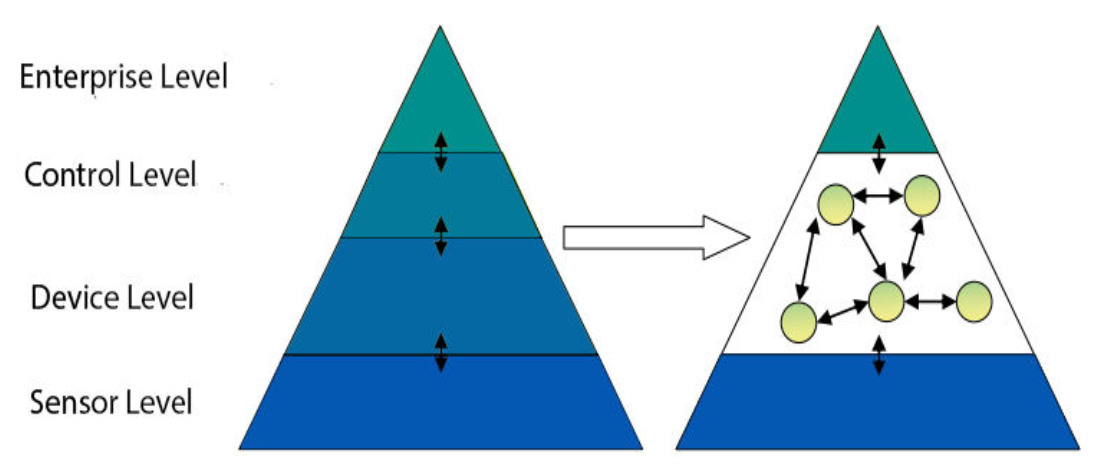
\includegraphics[scale=0.5]{Figures/reconfigurationpyramide}
\decoRule
\caption[Change of industrial pyramide]{sfasdfasdf}
\label{4DIAC IDE System Perspective}
\end{figure}

%----------------------------------------------------------------------------------------
%	Aim of thesis
%----------------------------------------------------------------------------------------

\section{The aim of thesis}
The aim of this thesis is to integrate OPC UA communication protocol into the system 4DIAC - controlling framework based on IEC 61499 standard. 

Controll system created in 4DIAC framework is composed by the function blocks, my task is to implement communication stack inside of function blocks. Including client and also server. 

OPC UA protocol allows user to create topologically ordered web of data. My work also aims to create data topology on the server based on a structure of the control system based on a 4DIAC framework. By the integration of these two technologies, I want to create a system in which all elements of distributed control system could load structure and status of every other element using OPC UA protocol. 



%----------------------------------------------------------------------------------------
%	Chapters overview
%----------------------------------------------------------------------------------------

\section{Chapters overview}
Aim of the following second chapter is to introduce you a IEC 61499 standard and 4DIAC framework based on this standard.
Basic principles of this framework as creating application, function blocks, deploying applications is described.
Important part of using 4DIAC framework is the compiling of your own version of 4DIAC runtime environment dedicated for your device. The whole appendix is dedicated to this topic.

The third chapter is dedicated to communication protocol OPC UA, ways of using this protovol and its information model. I am going to mention stacks based on OPC UA protocol. I am focusing on OPEN 62541 stack, which i have chosen to use in this thesis. 

In the fourth chapter I am explaining my solution of the problem explained in the previous sections of this chapter. Also I am describing the example application to work with OPC UA in 4DIAC.





% Chapter Template

\chapter{IEC 61499} % Main chapter title
\label{Chapter2} % Change X to a consecutive number; for referencing this chapter elsewhere, use \ref{ChapterX}

%----------------------------------------------------------------------------------------
%	SECTION 1
%----------------------------------------------------------------------------------------



IEC 61499 is a new family of standards for Industrial Process Measurement and Control Systems (IPCMCS). This family consist of four parts:

\begin{enumerate}
	\item IEC 61499-1 : Function Blocks - Part 1: Architecture
	\item IEC 61499-2 : Function Blocks - Part 2: Software tools requirements
	\item IEC 61499-3 : Function blocks for industrial-process measurement and control systems - Part 3: Tutorial information 
	\item IEC 61499-4 : Function Blocks - Part 4 : Rules for compliance profiles
\end{enumerate}


Main purpose of all parts of this family is to define Function Block (FB), so in this Thesis term IEC 61499 refer to the whole family of these standards. 
IEC 61499 is based on an older IEC 61311 (1993) family of standards, which is the most common adopted standard in domain of IPMCS.  (citovat Aloisa)
This makes IEC 61499 easy to adopt. There are also another key features which makes IEC 61499 easy to adopt standard like its modularity, distribution support, reconfiguration support and event-triggered execution model. 

\section{Introduction to IEC 61499}

The IEC 61499 standard defines several models, which  developer uses to create a distributed control application in a graphical manner. This brief introduction will give you insight into the IEC 61499 standard for purposes of this thesis. A full description of architecture may be found in IEC61499-1.

Models which are defined in IEC 61499 are (in hierarchical order, from the global model to atomic one): the application model, the system model, the device model, the resource model, the Fucntion Block (FB) model.

The application model consists of the multiple system models, one of these system models consist of multiple device models etc. 

The Base and most important model of IEC 61499 is FB. FB is independent, self-contained software component with the interface through which it provides specific functions. This model was taken from IEC 61131-3 standard. Against IEC 61131-3 FB definition in IEC 61499 event interface is added. The function block function is triggered by one of the input events. During the execution FB processes input data, set output data. When the processing is done FB generates triggers output event. 

\begin{figure}
\centering
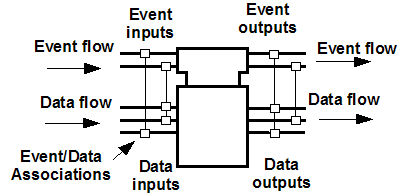
\includegraphics{Figures/IEC61499FunctionBlock}
\decoRule
\caption[IEC 61499 Function Block]{http://www.automation.com/images/isa_automation_week/IEC61499FunctionBlock.png}
\label{fig:IEC61499FunctionBlock}
\end{figure}
 

When comparing IEC 61131-3 and IEC 61499 the biggest difference is in the even-driven execution, while in IEC 61131-3 function was triggered by the cyclic execution.

Cyclic execution was problematic. It does not allow mass using of IEC 61131-3 in distributed systems. This type of execution is 	reliant to the system clock. This approach is not problematic in the scope of one device system. However, in the system with multiple devices there is a problem of sharing the system time. It is practically impossible to run this kind of system synchronously.
In case of the cyclic execution every 1ms and not precise synchronous system it can take up to 1ms to handle any kind of change. In some kind of applications this time delay can lead to the destruction of product, machine or even whole manufacturing system. 
This problem can be solved by decreasing time between two executions. However this solution of delay problem is causing need of bandwidth for data transfer. It leads to the cost of data transport layer increase and also scale up data transfer error rate possibility. 

In IEC 61499 standard this problem was solved by changing cyclic to event driven execution. Function Blocks are not executed cyclically, but are triggered by event. This solution prevents problem with the central time and its sharing and caused also rapid decrease of needed bandwidth. In this approach the data are transferred only when event is triggered. 
For example function block handling the end switch of machine does not have to propagate its state every 1ms like in the previous example. It propagates its state only when change state event occurs. 

There is no support in IEC 61499 for cyclic execution anymore, but for purposes of back compatibility there is a solution of implementing IEC 61131 function into IEC 61499 system. The situation of a program is simply depicted by triggering of the cyclic execution by the use of an E\_CYCLE FB.\cite{4618109} This function block triggers regular event to start execution of IEC 61131-3 compatible applications. 

\section{Types of FB in IEC 61499}

\subsection{Basic FB}
Basic FB (BFB) contains a state machine controlling internal execution called Execution Control Chart (ECC).
ECC consists of three parts: ECC states with associated ECC actions and ECC transitions, which connects the states. ECC transitions are typically guarded by Boolean logical statements. 

When an input event arrives, the first transition with true condition results in state change. With state entry also action associated with this state is executed. Algorithm can access only data input, data output and inner variables. //citovat IEC 61499-1

\begin{figure}[hbp]
\centering
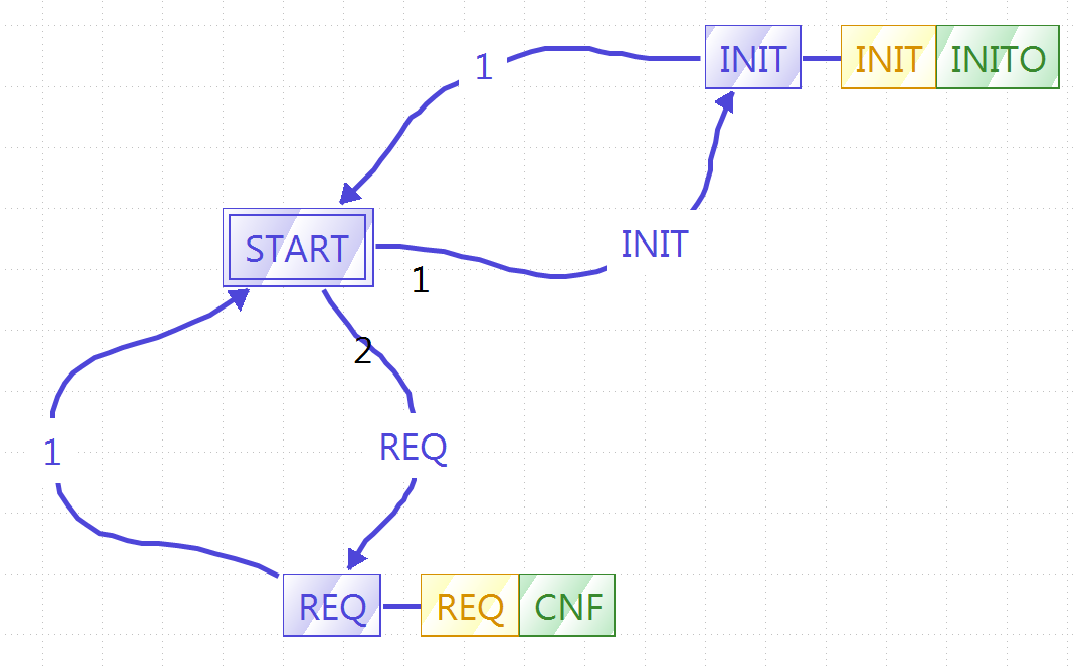
\includegraphics[scale=0.5]{Figures/basicfb-ecc}
\decoRule
\caption[IEC 61499 Basic FB's ECC]{Example of basic FB's ECC}
\label{IEC 61499 Basic FB's ECC}
\end{figure}

\subsection{Composite FB}


Composite FBs (CFBs) are containers for FB dedicated to generate cleaner design. Using Composite FBs developer can create one FB for more complex, many times repeating function consisting of many basic or composite FBs. This allows designer to re-use his design. 
Incomming event and data connections are connected to the internal FBs and also outgoing connections are connected to internal FBs.


\begin{figure}[hbp]
\centering
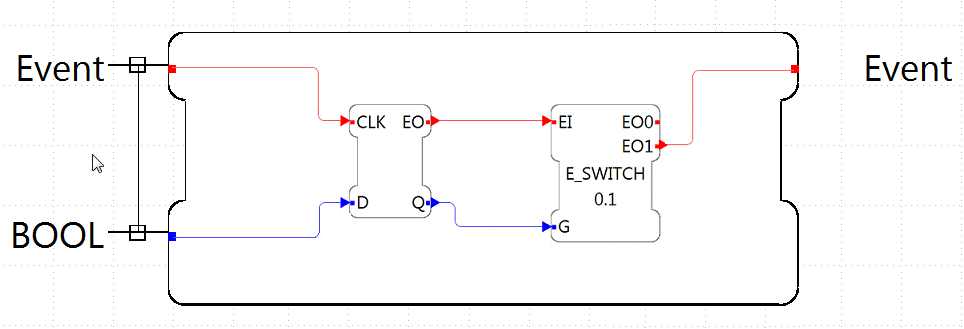
\includegraphics[scale=0.5]{Figures/compositefb}
\decoRule
\caption[IEC 61499 Composite FB]{Example of composite FB structure}
\label{IEC 61499 Composite FB}
\end{figure}

\subsection{Service Interface FB}
Service Interface FB is dedicated to function out of scope of IEC 61499. Typical function is the access to the device's hardware, I/O interface or communication interface. There are two general types of SIFBs in IEC 61499. Requester SIFB and responder SIFB. The requester SIFB remains passive, until it is application-triggered at one of its event inputs. 
The responder type is a resource or hardware triggered FB. It can trigger events by detecting actions of the hardware (e.g. interrupts) without need to trigger this FB from application. 

\section{IEC 61499 Base Model}

Modeling of IEC 61449 system can be divided into two phases. 
In the first phase designer creates Function Block Network by interconnecting of the FBs with data and event connection. In this phase developer has in mind only functionality and it does not depend on any device or control infrastructure. 
In the second phase parts of the system model created in the first phase are mapped to control devices.
For example, in Figure 2.4a, Application 1 is mapped to Devices 2, 3, 4, and 5, whereas Application 2 is mapped only to device 2. 

\begin{figure}[hbp]
\centering
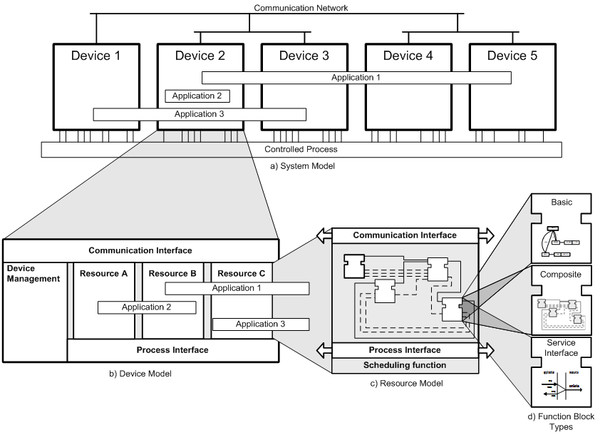
\includegraphics[scale=0.6]{Figures/IEC61499Models}
\decoRule
\caption[IEC 61499 Base Model]{http://2.bp.blogspot.com/-qzJhgeMHSnQ/UNZC7b0op6I/AAAAAAAALwk/aW3FpwY3e5o/s1600/IEC+61499+Models.jpg}
\label{IEC 61499 Base Model}
\end{figure}

IEC 61499 is executed on devices. Every device consist of device management component, communication iterface - provides communication between devices, process interface - provides services for accessing the sensors, actuators and other physical devices needed to control the process. Device can also contain resource. 

Resources are functional units which contain applications or the  parts of applications. Resources in device are independend. This means resources can be added, modified, removed in any particular device without interferring any other resource. This approach is very important to reach the goal of reconfiguration. The task of the resource is to provide execution environment, delivering event notifications.

\section{IEC 61499 applications}
The current application of IEC 61499 can be devided into the research and industrial sector.
IEC 61499 standard exists since January 2005. Before standardization in 2000 it was available in form of so-called Public Available Specification. Although IEC 61499 has been available in some forms for a long time, most published work on the standard up to now has been academic or, if industrially-based has resulted only in prototypical test cases.\cite{4618110}

In industry sector the adoptions of IEC 61499 were mainly case studies and prototypes. A lot of case studies had a starting point via FBDK/FBRT package from Rockwell Automation.
FBRT is implemented in Java and IEC 61499 elements are implemented as Java Classes. This package is a reference implementation and was used to test models and standard. In FBRT the event notification is handeld by function call. The source FB calls notification function of the event connection object and this object triggers event on destination FB by calling his event function. This approach creates delays and is also one of the greatest reasons why FBRT has never been adopted by industry sector. Another reason is also that this Java implementation was not able to run on small industrial control platforms (8/16/32b computers). 


\section{The 4DIAC initiative}

In July 2007 the 4diac open source initiative was founded by PROFACTOR GmbH and the Automation and Control Institute of Vienna University of Technology. 
Nowadays this initiative is conducted with and supported by international automation network O\footnote{3}NEIDA. 


Aim of 4DIAC initiative is to create an open-source framework based on IEC 61499 standard which will provide reference implementation of execution model for IEC 61499.

4DIAC initiative is currently developing two projects IEC 61499 compliant :
\begin{itemize}
	\item 4DIAC IDE - engineering tool
	\item FORTE - runtime environment
\end{itemize}

To work with 4DIAC framework you have to use both of this parts. 

You can find instructions how to install and run this project on your own computer in Appendix A. 
In the next sections brief informations about 4DIAC IDE and FORTE are introduced. These are just the minimal amount of necessary informatios in needs of this thesis.

\section{4DIAC IDE}

4DIAC IDE is IEC 61499 development evironmen based on the Eclipse open tool framework. 
Eclipse base makes 4DIAC IDE multiplatform open source IDE. 

As all other IDEs based on Eclipse work in 4DIAC IDE is divided into perspectives. Every user can create his own perspective, but there are three perspectives which are created by default in 4DIAC IDE. 

This perspective is dedicated to the basic creation of application. FBs can be added, created event and data connection. Below system configuration of one of the example supplied with 4DIAC IDE can be seen. 

Application of figure consist of two devices, connected via Ethernet. Every of this device includes two resources. One of the resources is management resource allways named MGR and read-only.

\begin{figure}[hbp]
\centering
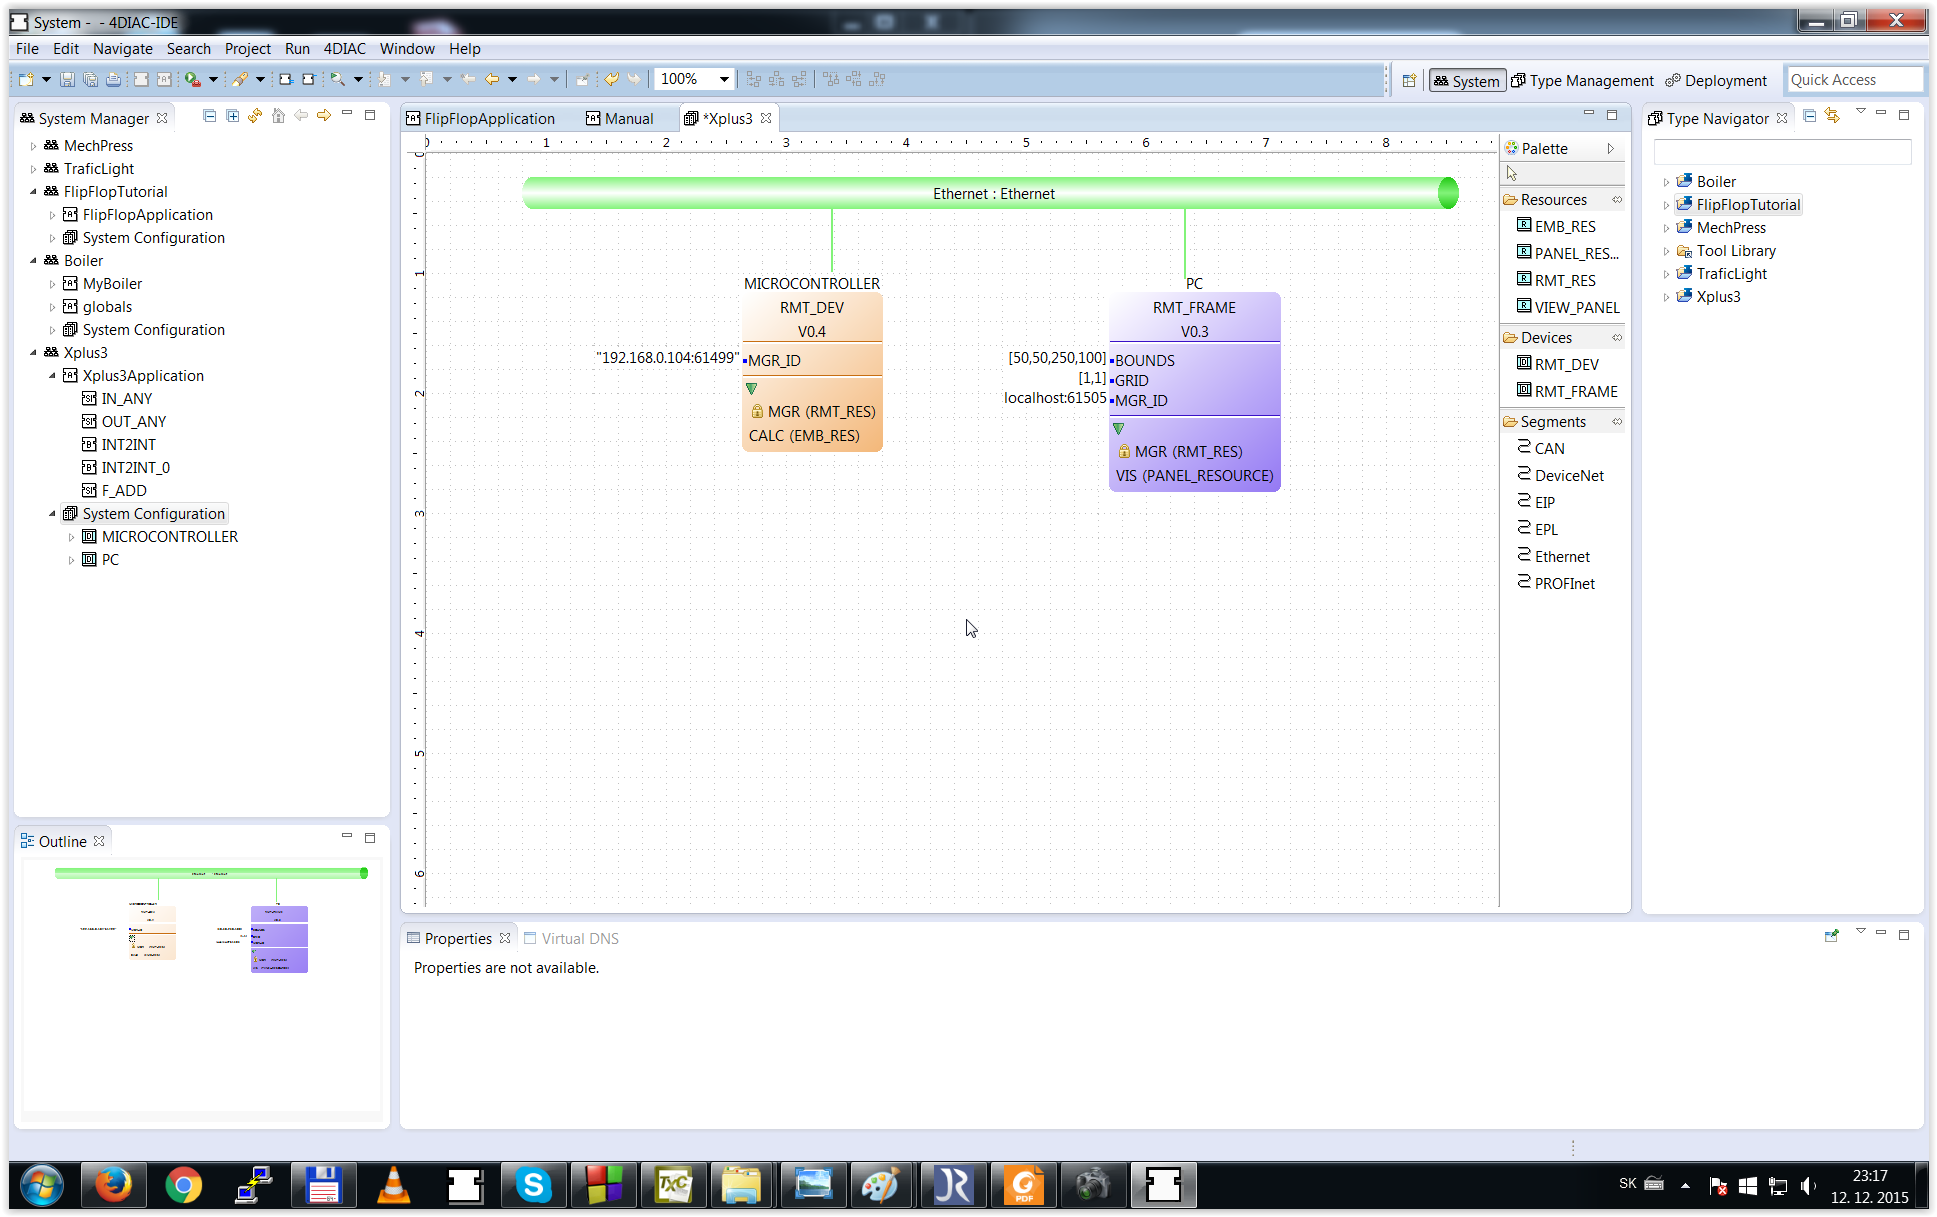
\includegraphics[scale=0.3]{Figures/systemperspective}
\decoRule
\caption[4DIAC IDE System Perspective]{Perspective dedicated to basic creation of application}
\label{4DIAC IDE System Perspective}
\end{figure}

By double clicking on resource you can edit Function Block Network running on this resource.

\begin{figure}[hbp]
\centering
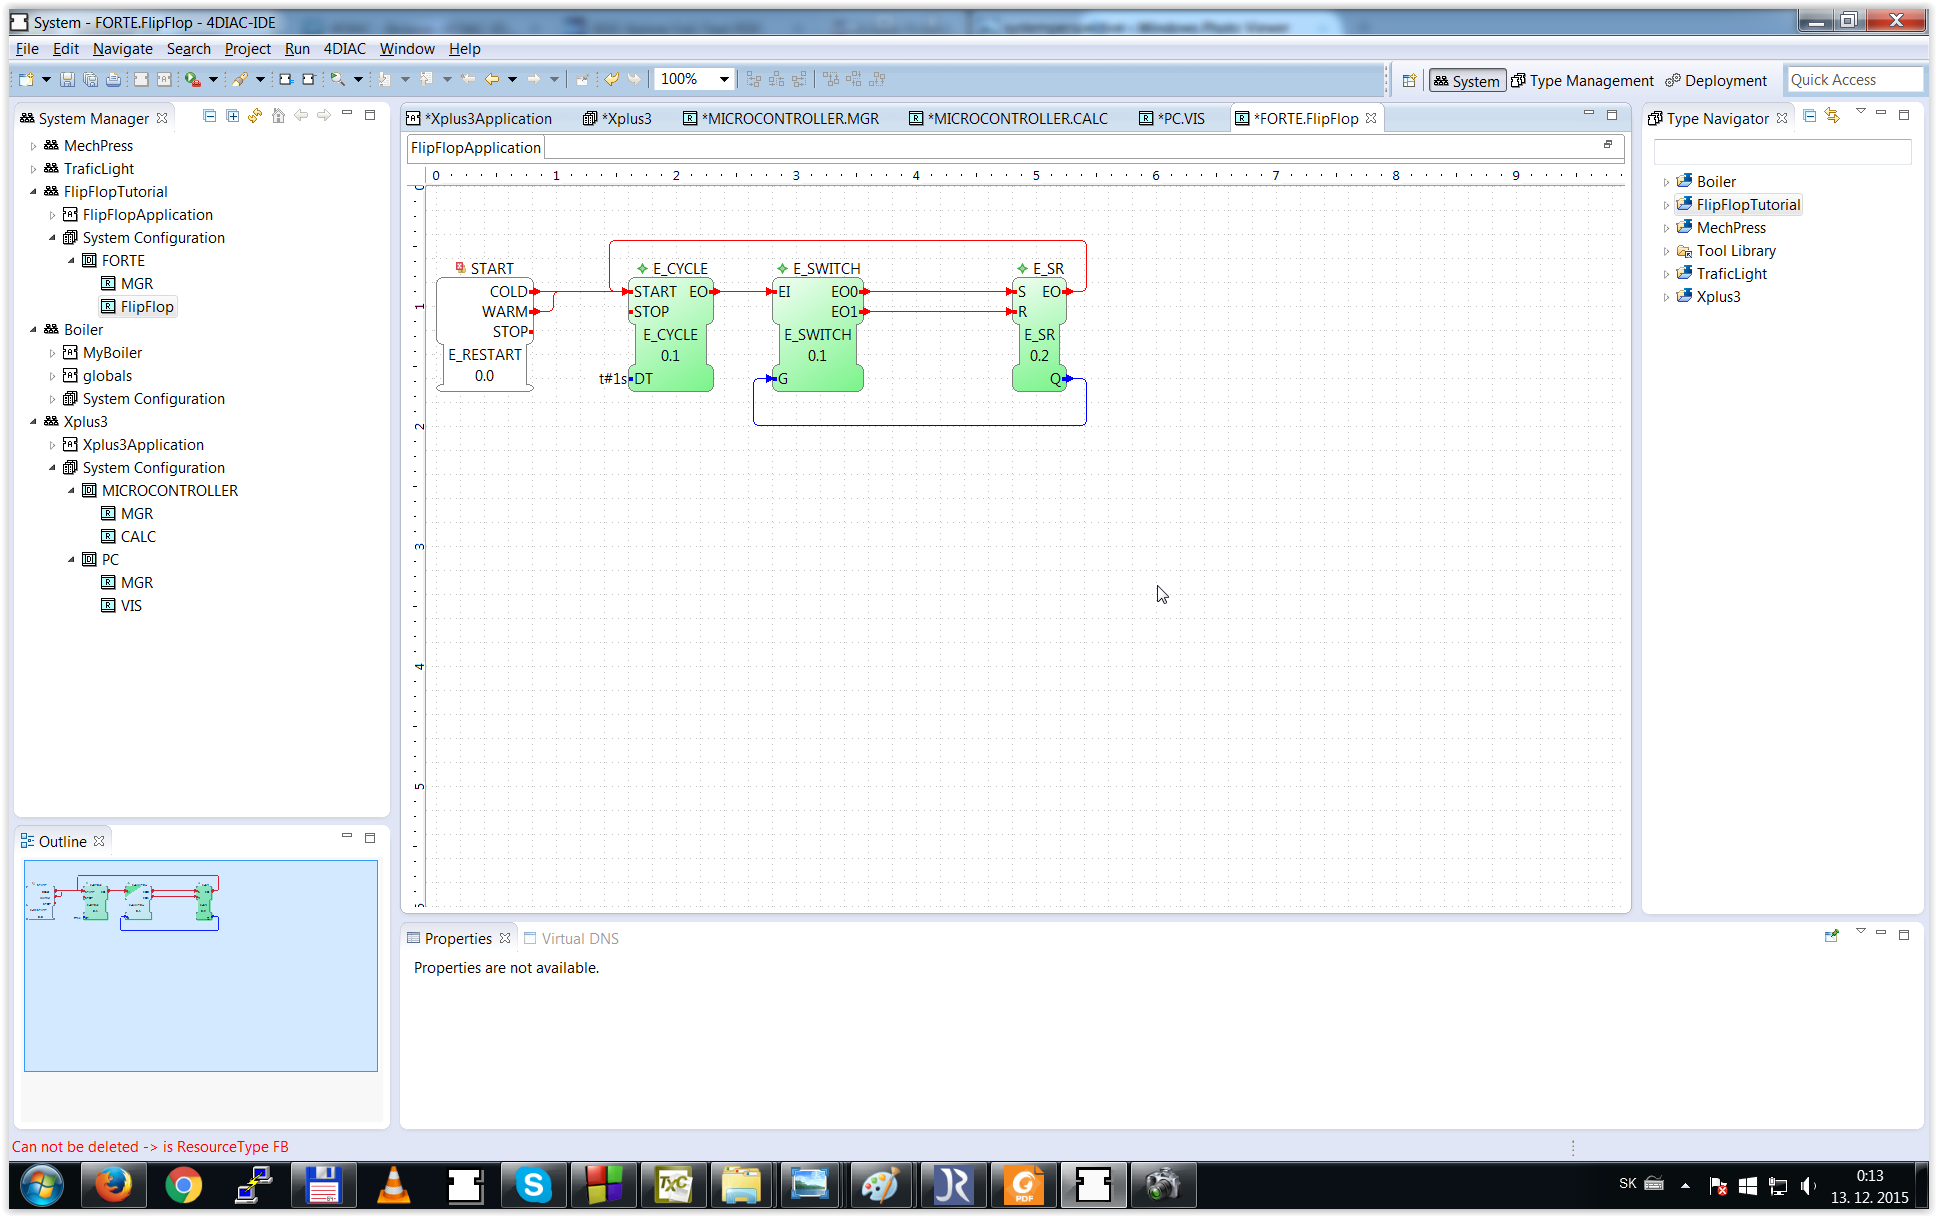
\includegraphics[scale=0.3]{Figures/systemapplicationperspective}
\decoRule
\caption[4DIAC IDE System Perspective - Resource]{Editing Function Block Network in resource}
\label{4DIAC IDE System Perspective - Resource}
\end{figure}

Type Management Perspective is dedicated to editing and creating of developers' own FBs. 
On the figure below, there are shown tools which can be applied on the function block.
In the case of the basic FB you can edit also function of this FB by editing its EEC or Algorithm writen in pseudocode. 
The function of the Composite FB can by modified or created by editing Composite Network. Only Service Interface FBs function is not allowed to change in 4DIAC editor. Function of SIFBs can be modified only by editing forte source. 

All changes made in Type Management Perspective have to be exported into the forte code. To use this modified FBs in control system it is necessary to recompile the FORTE with these updated function block.


\begin{figure}[hbp]
\centering
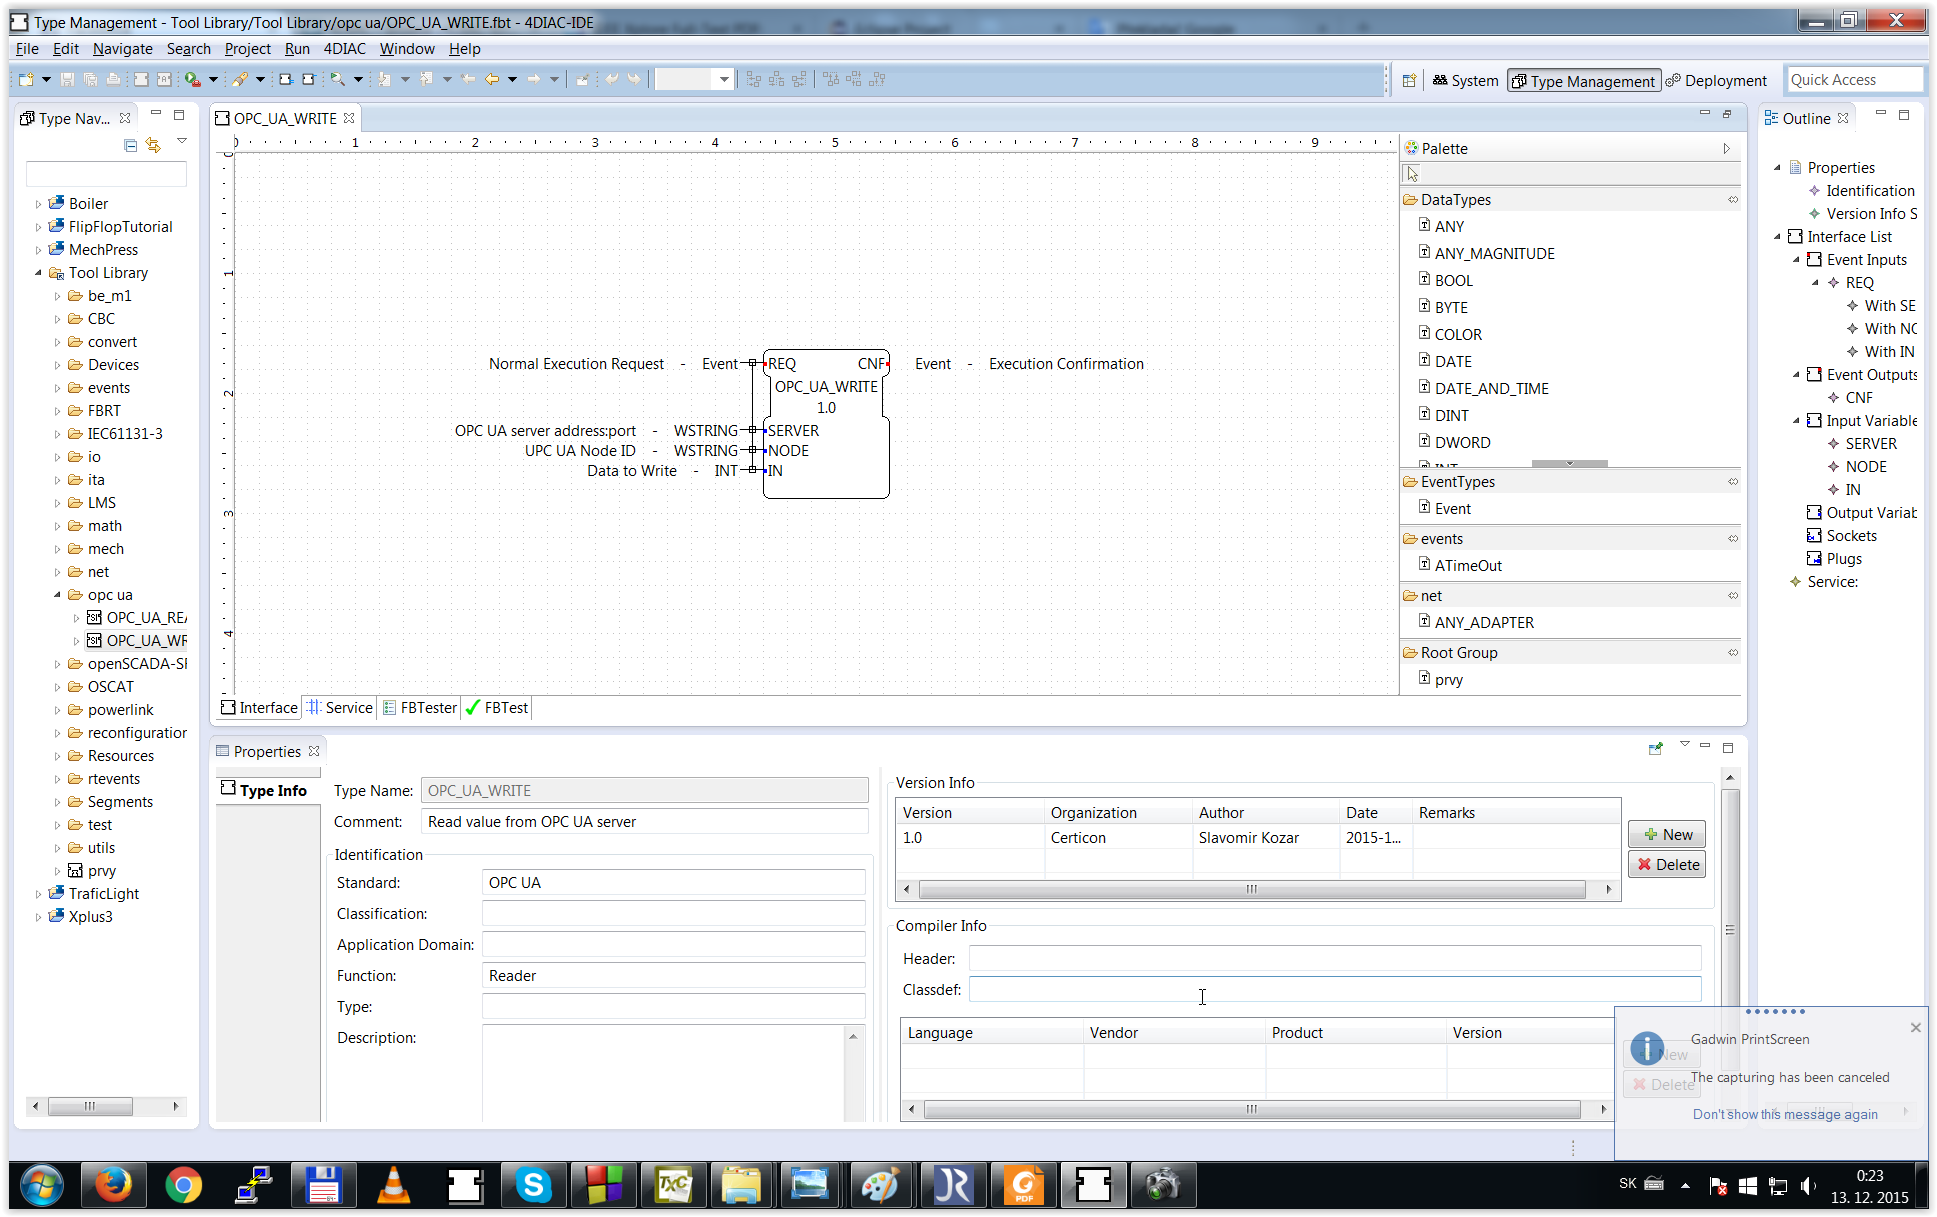
\includegraphics[scale=0.3]{Figures/typemanagementperspective}
\decoRule
\caption[4DIAC IDE Type Management Perspective ]{Editing or Creating FBs}
\label{4DIAC IDE Type Management Perspective}
\end{figure}


Deployment Perspective is dedicated to the deployment and upload application into the control system devices by clicking on Download button.

There is also possibility to run local FORTE and FBRT directly from Deployment Perspective. In case of local FORTE runtime, all its output are shown in Console window. 


\begin{figure}[hbp]
\centering
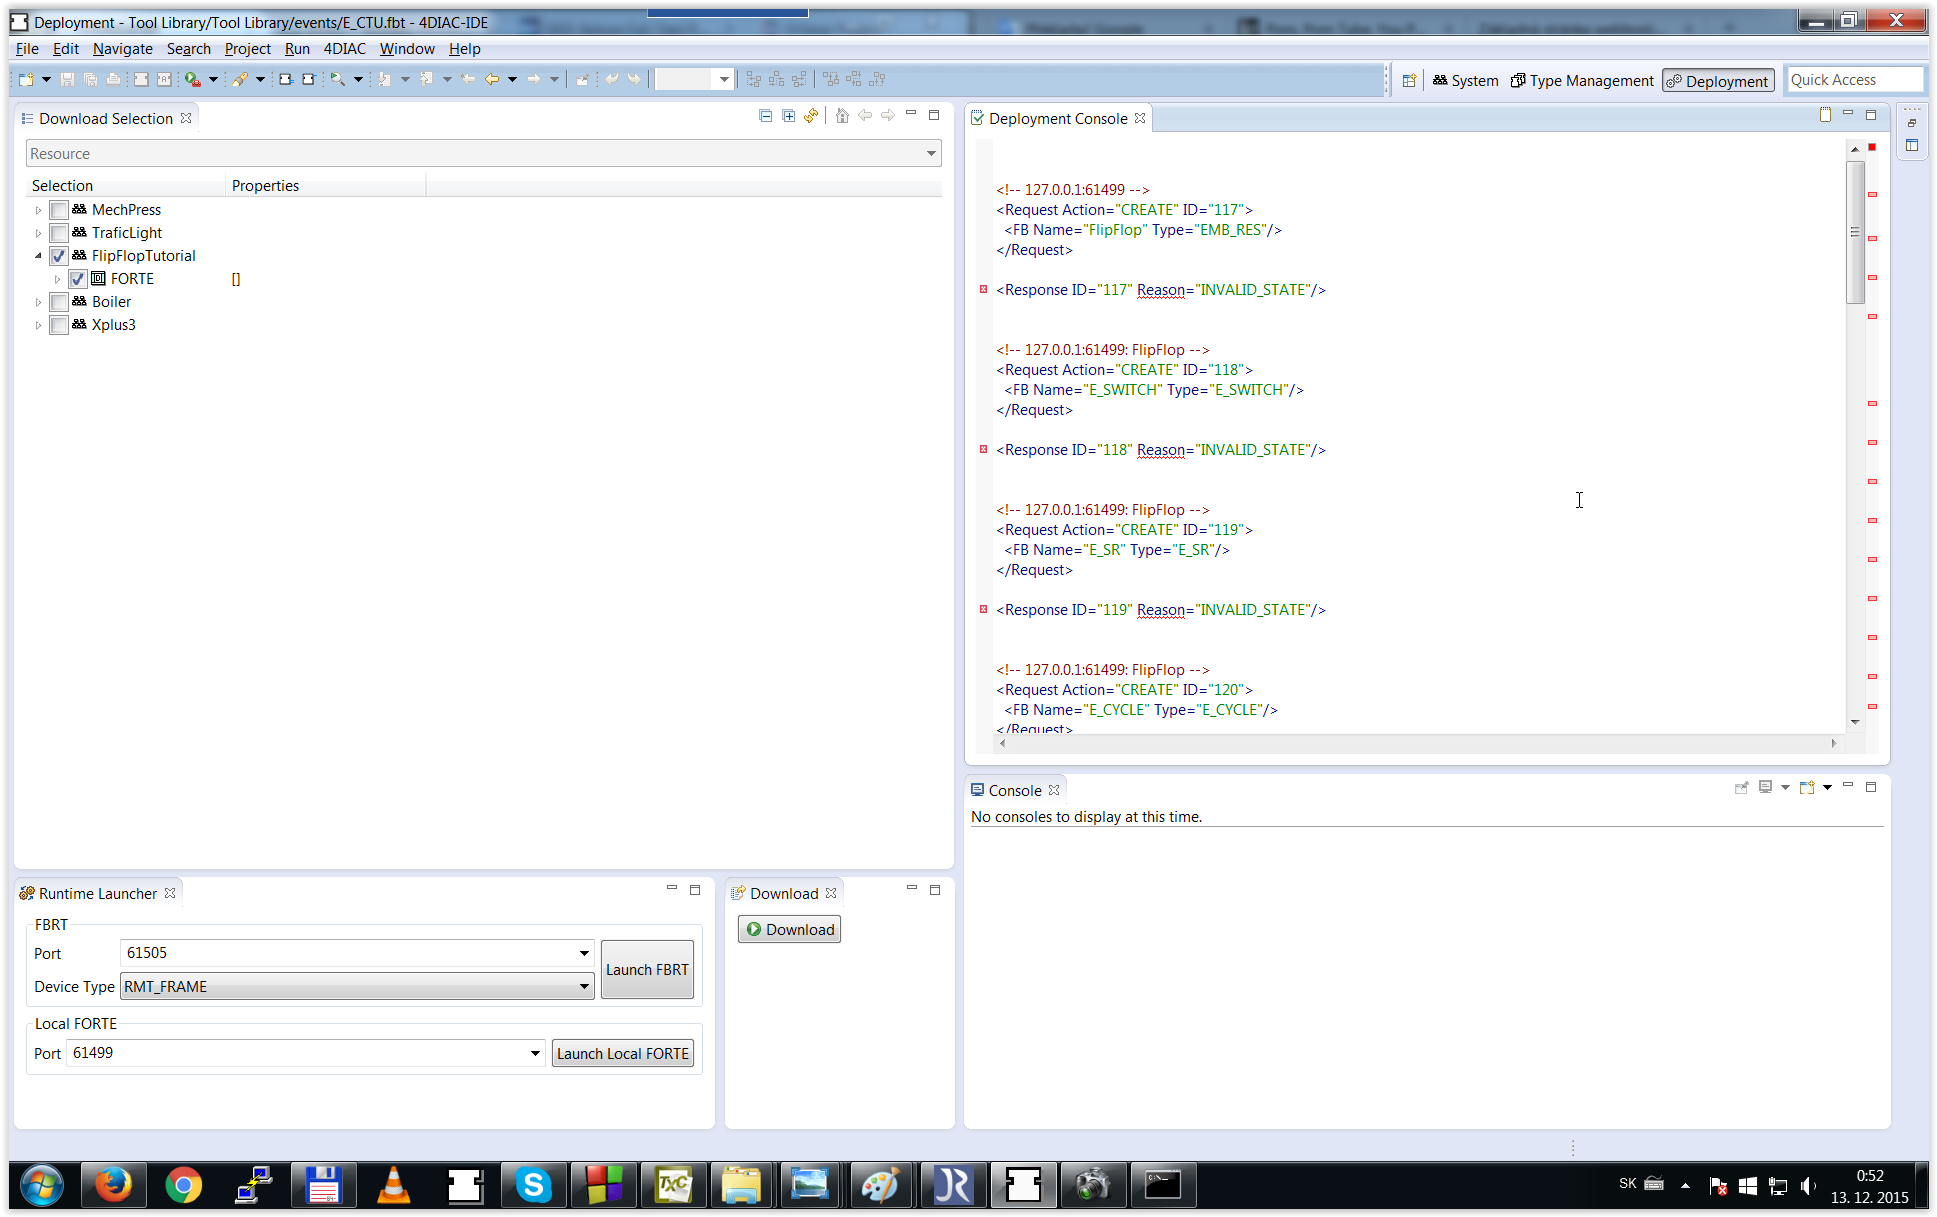
\includegraphics[scale=0.3]{Figures/deploymentperspective}
\decoRule
\caption[4DIAC IDE Deployment Perspective ]{Uploading application into devices}
\label{4DIAC IDE Deployment Perspective}
\end{figure}



\section{4DIAC RUNTIME ENVIRONMENT - FORTE}


The FORTE is a portable C++ implementation of an IEC 61499 runtime environment. It is focused on the small embedded control devices (also 16/ 32 bit controllers) and provides execution of all IEC 61499 types of functions blocks. Currently is forte available for Windows, Posix (Cygwin, Linux), NET+OS 7, eCos. It can be also used on small embedded boards like RaspberryPi, BeagleBone or even Lego Mindstroms nxt. 

\subsection{Function Blocks in the FORTE}
Basic and composite FBs are easy to create and edit in 4DIAC IDE. 
However Service Interfaces FBs, which are most important, because serves connection to the physical devices in control system are defined twice. 
In 4DIAC IDE only outer interface, like event and data inputs outputs are defined function of these function blocks is defined in C++ function generated to every function block. Creating of function block will be discussed in the next chapters. 


 
% Chapter Template

\chapter{OPC Unified Architecture} % Main chapter title

\label{Chapter3} % Change X to a consecutive number; for referencing this chapter elsewhere, use \ref{ChapterX}

%----------------------------------------------------------------------------------------
%	SECTION 1
%----------------------------------------------------------------------------------------

\section{Service Oriented Architecture}

Service Oriented Architecture is family of principles which recommends assembling of the composite application and any other systems from the independend parts servicing any kind of the service. 

Nowadays most of the information technologies are moving into web. With incomming Internet of Things into industry, this section is not an exception. 
Anyhow industrial applications may differ a lot from each other, there is tendency to connect them together to create a larger systems. Main connection between different systems is the SOA, principes which can connect technologies on a different platforms. This technology transfer alone control and regulation systems into the global solutions. 


On figure below is obvious how SOA converts monotlitic and not-scalable system into the much more clear solution. Creating of the same application using single atomic services leads into the system which is much more scalable, reconfigurable and independent modules servicing data supports also much more debugging abilities of service without need to shut down the whole system.

\begin{figure}[hbp]
\centering
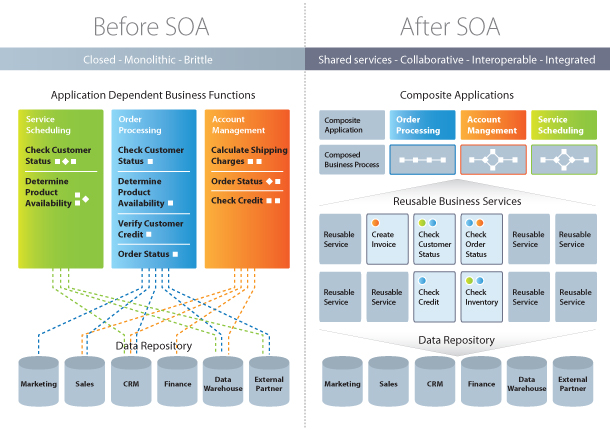
\includegraphics[scale=0.3]{Figures/diagram-soa}
\decoRule
\caption[4DIAC IDE Deployment Perspective ]{http://www.tridens.si/wp-content/uploads/2010/04/diagram-soa.jpg}
\label{4DIAC IDE Deployment Perspective}
\end{figure}


This approach brings re-usability feature, which is whole common in the other IT sectors, into the industrial systems.


\section{Web service}


Web service is a software system for communication of two computers in the network. It is described in a Web Services Description Language (WSDL). A Web service supports direct interactions with the other software agents using XML-based messages exchanged via Internet-based protocols. \cite{raey} Often the web port 80 is used to transfer data. This port is used mainly by web http protocol, so is opened on almoust every firewall. That is the huge advantage against any kind of proprietal ports. 


%-----------------------------------
%	SUBSECTION 1
%-----------------------------------
\section{OPC Unified Architecture}

Information system exceeds the borders of plant or event company, when companies are working together on common projects and products.
Due the huge demand of integration and interconnecting different control system the standardization is needed. Standardization of information systems reduces cost and time of integration. With standards comes also possibility to create generic adapters between any kind of systems. 

OPC Foundation answers this need of standardization. 
In the begining the OPC standed for OLE for Process Control. The OLE itself is Microsof proprietary technology called Object Linking and Embedding. This technology is used by Microsof to create references between the data objects in Windows OS. Microsoft later published SDK for this technology which leads to creation of the OPC. 

OPC Foundation decided to redesign OPC components and technologies with modern, vendor independent solutions.\cite{4618203}


The new specification is called OPC Unified Architecture (OPC UA). Nowadays the OPC means Openness, Productivity and Colaboration.


Currently, OPC is the communication standard in automation technology. Migration to OPC UA is needed to increase possible types of the integration solutions for which UPC can be used. This is achieved by using standard technologies to implement SOA and WS. 

\subsection{SOA in OPC UA}
OPC UA is based on SOA. OPC UA server contains set of services which are used by clients. These services provides all OPC UA functionality. 
Set of services available in any particular OPC UA server is defined in profiles that are described in OPC UA specification.

Each service call in IPC UA consist of a request and response message. 
In OPC UA there is a huge difference between services and methods. Wile services are strictly defined in the standard and user cannot change it, methods are user defined.
To invoke user-defined method on OPC UA server using service needed. 

\subsection{OPC UA communication stacks}
All the OPC UA standards are published by the OPC UA Foundation, but no official communication stack has been published yet.
OPC Foundation published just the example code in Java and Ansi C, but no complete SDK or even documentation.

However there are few open source or proprietary stacks available. 
On http://www.opcconnect.com/uakit.php#overview you can find Overview of Available SDKs and toolkits. 

There are also some open stacks for OPC UA. However these stacks are often published under license which is not compatible with 4DIAC license. 
I can mention OpenOpcUa which is open source, but to use it there is need to pay the one time fee. I can also mention FreeOpcUa hosted by the GitHub, but this sdk is not fully working and lack of documentation makes it almous impossible to use it for purpose of this thesis. However FreeOpcUa is C/C++ and Python SDK and in Python version much bigger progress is made. This SDK serves great open-source Python GUI interface for discovering the OPC UA server. 

Considering two important parameters license and documentation, open62541 stack seems to be optimal. This stack is used to integrate OPC UA into FORTE and will be described more in the below sections.

%-----------------------------------
%	SUBSECTION 2
%-----------------------------------

\section{OPEN 62541 stack}
Open 62541 is communication stack based on OPC UA standards published as IEC 62541 licensed under LGPL and free available on GitHub.

This stack is fully scalable, supports multi-threaded architecture, where every connection or session is operated by separate thread.

Open 62541 is written in C99 with POSIX support, so it is able to run on Windows, Linux, MacOS and Android. POSIX Linux support means open 62541 stack can also run on small embedded machines like raspberryPi, PLCs, etc.


\subsection{building sdk}
After downlaoding open 62541 stack sources from GitHub it is necessary to build them into header files. Also pre-generated sources and header files are available to downlaod. This pre-generated sources are just some demo with only basic functions like server, client and its basic functionality like read and write data. In this thesis also another functions like browsing across nodes on server and creating, editing and deleting nodes were needed, so in order to fullfil aim og this thesis specific sources were build. 

For detailed information about building library visit oficial documentation of open 62541.
http://open62541.org/doc/current/building.html



%----------------------------------------------------------------------------------------
%	SECTION 2
%----------------------------------------------------------------------------------------


% Chapter Template

\chapter{Chapter Title Here} % Main chapter title

\label{ChapterX} % Change X to a consecutive number; for referencing this chapter elsewhere, use \ref{ChapterX}

%----------------------------------------------------------------------------------------
%	SECTION 1
%----------------------------------------------------------------------------------------

\section{Main Section 1}

Lorem ipsum dolor sit amet, consectetur adipiscing elit. Aliquam ultricies lacinia euismod. Nam tempus risus in dolor rhoncus in interdum enim tincidunt. Donec vel nunc neque. In condimentum ullamcorper quam non consequat. Fusce sagittis tempor feugiat. Fusce magna erat, molestie eu convallis ut, tempus sed arcu. Quisque molestie, ante a tincidunt ullamcorper, sapien enim dignissim lacus, in semper nibh erat lobortis purus. Integer dapibus ligula ac risus convallis pellentesque.

%-----------------------------------
%	SUBSECTION 1
%-----------------------------------
\subsection{Subsection 1}

Nunc posuere quam at lectus tristique eu ultrices augue venenatis. Vestibulum ante ipsum primis in faucibus orci luctus et ultrices posuere cubilia Curae; Aliquam erat volutpat. Vivamus sodales tortor eget quam adipiscing in vulputate ante ullamcorper. Sed eros ante, lacinia et sollicitudin et, aliquam sit amet augue. In hac habitasse platea dictumst.

%-----------------------------------
%	SUBSECTION 2
%-----------------------------------

\subsection{Subsection 2}
Morbi rutrum odio eget arcu adipiscing sodales. Aenean et purus a est pulvinar pellentesque. Cras in elit neque, quis varius elit. Phasellus fringilla, nibh eu tempus venenatis, dolor elit posuere quam, quis adipiscing urna leo nec orci. Sed nec nulla auctor odio aliquet consequat. Ut nec nulla in ante ullamcorper aliquam at sed dolor. Phasellus fermentum magna in augue gravida cursus. Cras sed pretium lorem. Pellentesque eget ornare odio. Proin accumsan, massa viverra cursus pharetra, ipsum nisi lobortis velit, a malesuada dolor lorem eu neque.

%----------------------------------------------------------------------------------------
%	SECTION 2
%----------------------------------------------------------------------------------------

\section{Main Section 2}

Sed ullamcorper quam eu nisl interdum at interdum enim egestas. Aliquam placerat justo sed lectus lobortis ut porta nisl porttitor. Vestibulum mi dolor, lacinia molestie gravida at, tempus vitae ligula. Donec eget quam sapien, in viverra eros. Donec pellentesque justo a massa fringilla non vestibulum metus vestibulum. Vestibulum in orci quis felis tempor lacinia. Vivamus ornare ultrices facilisis. Ut hendrerit volutpat vulputate. Morbi condimentum venenatis augue, id porta ipsum vulputate in. Curabitur luctus tempus justo. Vestibulum risus lectus, adipiscing nec condimentum quis, condimentum nec nisl. Aliquam dictum sagittis velit sed iaculis. Morbi tristique augue sit amet nulla pulvinar id facilisis ligula mollis. Nam elit libero, tincidunt ut aliquam at, molestie in quam. Aenean rhoncus vehicula hendrerit. 
% Chapter Template

\chapter{Results} % Main chapter title

\label{Chapter5} % Change X to a consecutive number; for referencing this chapter elsewhere, use \ref{ChapterX}

%----------------------------------------------------------------------------------------
%	SECTION 1
%----------------------------------------------------------------------------------------

\section{Created function blocks}

Lorem ipsum dolor sit amet, consectetur adipiscing elit. Aliquam ultricies lacinia euismod. Nam tempus risus in dolor rhoncus in interdum enim tincidunt. Donec vel nunc neque. In condimentum ullamcorper quam non consequat. Fusce sagittis tempor feugiat. Fusce magna erat, molestie eu convallis ut, tempus sed arcu. Quisque molestie, ante a tincidunt ullamcorper, sapien enim dignissim lacus, in semper nibh erat lobortis purus. Integer dapibus ligula ac risus convallis pellentesque.

\section{Implementation of function blocks}

%-----------------------------------
%	SUBSECTION 1
%-----------------------------------
\subsection{server}

Nunc posuere quam at lectus tristique eu ultrices augue venenatis. Vestibulum ante ipsum primis in faucibus orci luctus et ultrices posuere cubilia Curae; Aliquam erat volutpat. Vivamus sodales tortor eget quam adipiscing in vulputate ante ullamcorper. Sed eros ante, lacinia et sollicitudin et, aliquam sit amet augue. In hac habitasse platea dictumst.

%-----------------------------------
%	SUBSECTION 2
%-----------------------------------

\subsection{subscriber}
Morbi rutrum odio eget arcu adipiscing sodales. Aenean et purus a est pulvinar pellentesque. Cras in elit neque, quis varius elit. Phasellus fringilla, nibh eu tempus venenatis, dolor elit posuere quam, quis adipiscing urna leo nec orci. Sed nec nulla auctor odio aliquet consequat. Ut nec nulla in ante ullamcorper aliquam at sed dolor. Phasellus fermentum magna in augue gravida cursus. Cras sed pretium lorem. Pellentesque eget ornare odio. Proin accumsan, massa viverra cursus pharetra, ipsum nisi lobortis velit, a malesuada dolor lorem eu neque.

\section{Example application}
%----------------------------------------------------------------------------------------
%	SECTION 2
%----------------------------------------------------------------------------------------

\section{Main Section 2}

Sed ullamcorper quam eu nisl interdum at interdum enim egestas. Aliquam placerat justo sed lectus lobortis ut porta nisl porttitor. Vestibulum mi dolor, lacinia molestie gravida at, tempus vitae ligula. Donec eget quam sapien, in viverra eros. Donec pellentesque justo a massa fringilla non vestibulum metus vestibulum. Vestibulum in orci quis felis tempor lacinia. Vivamus ornare ultrices facilisis. Ut hendrerit volutpat vulputate. Morbi condimentum venenatis augue, id porta ipsum vulputate in. Curabitur luctus tempus justo. Vestibulum risus lectus, adipiscing nec condimentum quis, condimentum nec nisl. Aliquam dictum sagittis velit sed iaculis. Morbi tristique augue sit amet nulla pulvinar id facilisis ligula mollis. Nam elit libero, tincidunt ut aliquam at, molestie in quam. Aenean rhoncus vehicula hendrerit. 

%----------------------------------------------------------------------------------------
%	THESIS CONTENT - APPENDICES
%----------------------------------------------------------------------------------------

\appendix % Cue to tell LaTeX that the following "chapters" are Appendices

% Include the appendices of the thesis as separate files from the Appendices folder
% Uncomment the lines as you write the Appendices

% Appendix A

\chapter{Appendix Title Here} % Main appendix title

\label{AppendixA} % For referencing this appendix elsewhere, use \ref{AppendixA}

Write your Appendix content here.
%% Appendix A

\chapter{Appendix Title Here} % Main appendix title

\label{AppendixA} % For referencing this appendix elsewhere, use \ref{AppendixA}

Write your Appendix content here.
%\include{Appendices/AppendixC}

%----------------------------------------------------------------------------------------
%	BIBLIOGRAPHY
%----------------------------------------------------------------------------------------

\printbibliography[heading=bibintoc]

%----------------------------------------------------------------------------------------

\end{document}  
